\chapter{Frontier Exploration: Using Wi-Coverage}

\lhead{\emph{Frontier Exploration}}

\par In the previous chapter, we have discussed the frontier based exploration in detail. This chapter presents the implementation of Wi-Coverage using which the frontier allocation is performed using a single robot and multiple robots. In this work, ROS and its supported packages are used: rtabmap\_ros for visual SLAM and move\_base for motion planning. Later in the Chapter, the systems involved are described.
\par Usually a human must map the territory in advance, providing either the exact locations of obstacles (for metric maps) or a graph representing the connectivity between open regions (for topological maps). As a result, most mobile robots become unable to navigate efficiently when placed in unknown environments. Exploration has the potential to free robots from this limitation. According to \cite{17} exploration is described as the act of moving through an unknown environment while building a map that can be used for subsequent navigation. A good and reliable exploration strategy is one which satisfies the following:
\begin{itemize}
    \item It should guarantee the complete coverage of any given environment, i.e it should be complete.
    \item It should be realizable in the real world.
    \item The algorithm should be computationally efficient. In other words, it should not be processor hungry.
    \item It should warranty that the communication between robots should be as minimum as possible.
    \item It should be scalable to large environments.
\end{itemize}


%v2
\section{Assumptions}
In order to present our approach in its best way, few assumptions are made with no effect on the behaviour of the algorithm:

\textbf{Network}: Wi-Coverage is based on utilizing signal strength of signals from routers for better exploration. We assume that the environment consists of Wi-Fi routers or temporary beacons which emit radio waves. It is empirically validated that, in order to sense the exact signal strength at a position in the environment, the receiver is expected to stay at that position for atleast 30secs. In all our simulations, the assume the bot receives the right signal strength in 15-20secs.  
-60dB is practically the least power which a general receiver can hear. In our simulations, if a signal listened to is less than -60dB, it is considered unheard. Similarly, any power higher than 20dB is considered 100\% received signal strength.  

\textbf{Robot}: Another assumption is that the robot is equipped with a static sensor. In other words, the sensors are fixed on the robot and don't move while navigation.

\textbf{Environment}: We do not take into account any noise or radio disturbances in the exploration space. Also phenomenons such as multi-path effect and Rayleigh fading are ignored. The ITU propagation model considers these effects to some extent. 

\section{Wi-Coverage}
\lhead{\emph{Wi-Coverage}}
Autonomous exploration has been a focus for many researchers in the field of robotics due to several reasons. One of them is that, tasks required for exploration are derivatives of the coverage problem wherein the main principle behind is to completely cover the area of a given environment. Several works discussed in Chapter 3, do not guarantee to solve the coverage problem. In other words, they are probabilistically complete or incomplete. Since the coverage problem can be time sensitive, the main evaluation metric for a solution is the amount of time required to successfully cover completely an environment.
\par There are several approaches in picking which frontier to select as the robots' next best location. In this implementation we use information gain as the criteria to decide the goal frontier and this is repeated until all the frontiers are exhausted, i.e until the environment is totally explored. But coverage of the environment is controlled using Wi-Coverage algorithm which clusters the environment using signal strengths from the surrounding Wi-Fi routers such that the robot covers the entire space cluster by cluster without any additional or prior information regarding the environment.

\section{Identifying frontiers}
As the robot does its initial sensor scan of its immediate environment, we obtain the occupancy grid (see chapter 2) using RTAB-Map package. Fig 3.1 below shows an example of the occupancy grid obtained in a simulation environment. The top view of the occupancy grid is a snapshot from Rviz, a visualization tool for ROS. The blue area represent the extent of the occupancy grid in the world. The black circle in the center is the Turtlebot simulated in Gazebo (see chapter 4). The grey portions of the occupancy grid seen have a probability of occupancy $p(m_i) = 0$ i.e the grid cells are empty or free. The black lines on grid have a probability of occupancy $p(m_i) = 1$ i.e those cells are occupied and represent the obstacles in the world shown in Fig 3.1(A). Finally the remaining portions on the occupancy grid in pale blue have a probability of occupancy $p(m_i) = 0.5$, meaning the uncertainty is maximum. Hence, they are the unknown cells of the map and are to be explored. The value $v(m_i)$ represents the type of cell. 0 being empty, 100 being occupied and -1 being unknown. Let O be the set of cells in a 2D occupancy grid and can be expressed as,

\begin{equation}
    O = \{c^{[xy]} : p(c^{[xy]}) = p' , p' \in [0.5,0,1]\}
\end{equation}
\begin{figure*}
    \begin{subfigure}[b]{\textwidth}
		\centering
		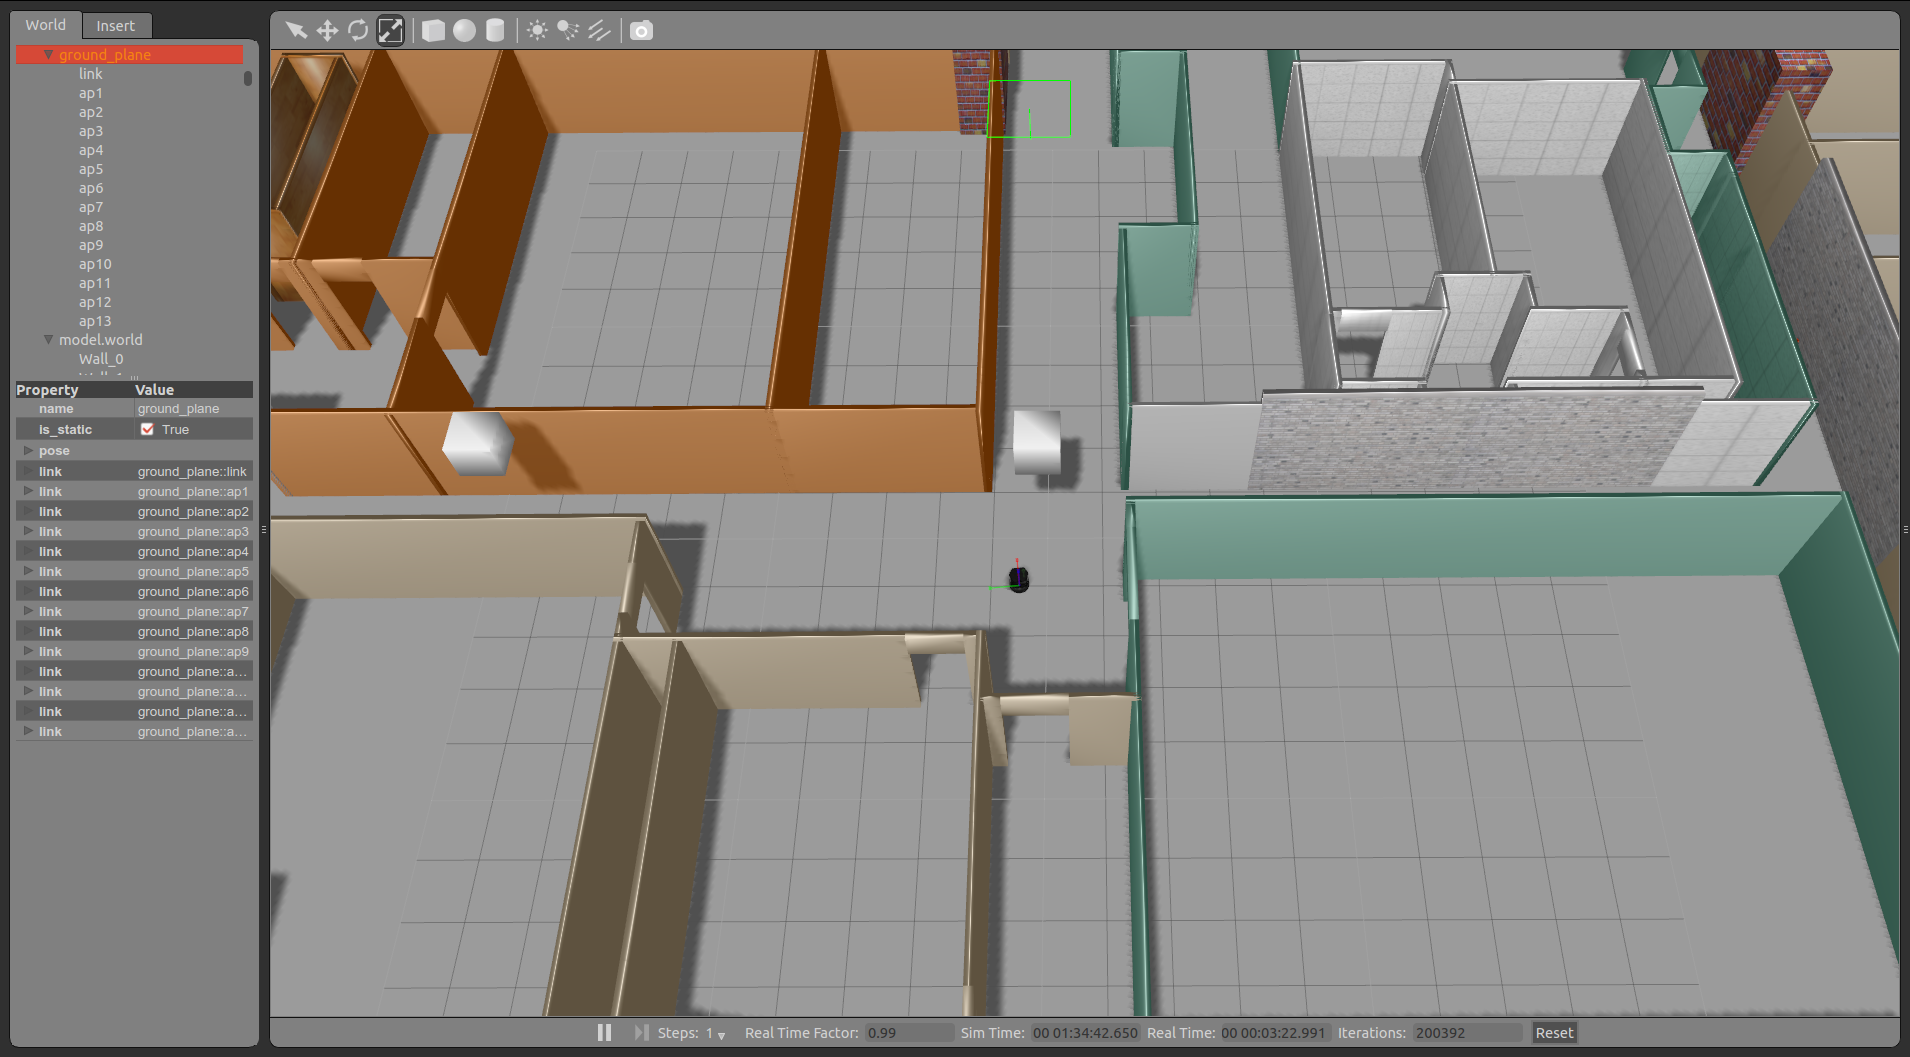
\includegraphics[width=\textwidth]{images/gazebo.png}
		\label{subfig:a}
		\caption{}
		\vspace{2em}
	\end{subfigure}
	\begin{subfigure}[b]{\textwidth}
	    \centering
		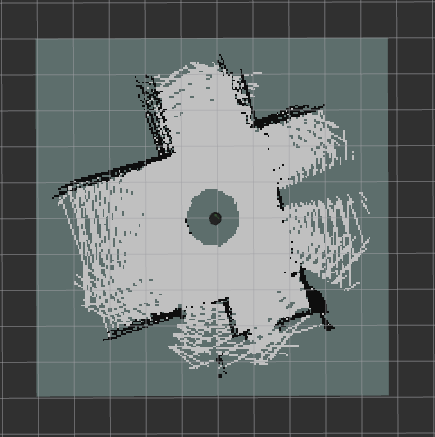
\includegraphics[width=0.75\textwidth]{images/gazebo1.png}
		\label{subfig:b}
		\caption{}
	\end{subfigure}
\caption{(A) Shows a simulation environment of Davis Hall, UB, created using Gazebo simulator for this work. (B) Shows the occupancy grid obtained from the vision sensor using RTAB-Map through topic /map\_explore.}
\end{figure*}

\par The consequent challenge is to identify the frontiers in the occupancy grid. As a part of solving an engineering issue discussed at the end of this chapter, we create a low resolution occupancy grid from the actual one every time it updates and frontiers are identified using the custom occupancy grid. Frontier is the boundary between explored i.e the grey cells and unexplored i.e the light blue cells. Each empty cell $v(m_i)=0$, is searched for at least one unknown cell $v(m_i)=-1$ adjacent to it and if found the cell is marked as a frontier cell given by,
\begin{equation}
    F = \{c^{[xy]} | c^{[xy]} \in O, \exists c^{[(x+m)(y+n)]} : p(c^{[(x+m)(y+n)]})=0.5, m\in[-1,1], n\in[-1,1]\}
\end{equation}
% The following the pseudo code to identify the grid cells which form the boundary separating the unknown from the free/empty space. 
The compute\_frontiers method in the controller.py node subscribes to the /map\_explore topic published by mapping.launch of RTAB-Map and detects the frontier cells.

\section{Information gain}
Entropy is the measure of uncertainty or randomness. Conditional entropy is defined as the entropy of a conditional distribution\cite{15}. The motto of exploration is to minimize the expected entropy of the belief as quickly as possible. As discussed in chapter 2, the following computes the expected entropy at a grid cell. 

\begin{equation}
    H = -\sum_{c^{[xy]}}[p(c^{[xy]})log_p(c^{[xy]}) + (1-p(c^{[xy]}))log(1-p(c^{[xy]}))], where~c^{[xy]} \in F
\end{equation}

We now calculate the cost for visiting each frontier cell. The cost in our case is simply the euclidean distance between robots position r and the target cell and is given by,

\begin{equation}
    \|C\|_{[xy]} = d(c^{[xy]},r^{[xy]}), where~c^{[xy]} \in F
\end{equation}
The optimal information gain associated with each frontier cell is defined as the difference between the expected entropy at it and the cost to visit it and is given by

\begin{equation}
    G_{[xy]} = H_{[xy]} - C_{[xy]} 
\end{equation}

\section{Frontier Allocation}
This work presents a new frontier allocation strategy which uses signal strengths from Wi-Fi routers. The proposed strategy is compared with another benchmark frontier allocation like optimal gain which are discussed in chapter 2. Wi-Coverage based frontier allocation provides a systematic coverage compared to the other approach.

\par To describe Wi-Coverage algorithm we consider two APs with access point IDs AP1 and AP2. We assume these APs are placed in an empty, obstacle free space as shown below in Fig 3.2. The rectangle with solid outline is the test environment and small green cubes represent the APs. Blue dotted circular outlines represent the reach of each APs and the dotted line between them divides the regions of AP dominance assuming such signal strength model. In other words, if the robot sensing Wi-Fi is in the region right to the line, it senses a stronger signal from AP1 than AP2. Similarly if it moves over the line towards AP2, it understands that the current region is dominated by AP2 than other APs which is only AP1 in this case. It is this ability to sense the dominance of APs in every region of the environment which forms the basis of Wi-Coverage of clustering the space online i.e. without any prior availability of clustered regions. The dividing line shown is only for illustration purposes and no such information about APs or the environment is required for Wi-Coverage. 

\begin{figure*}
    \begin{subfigure}[b]{0.495\textwidth}
		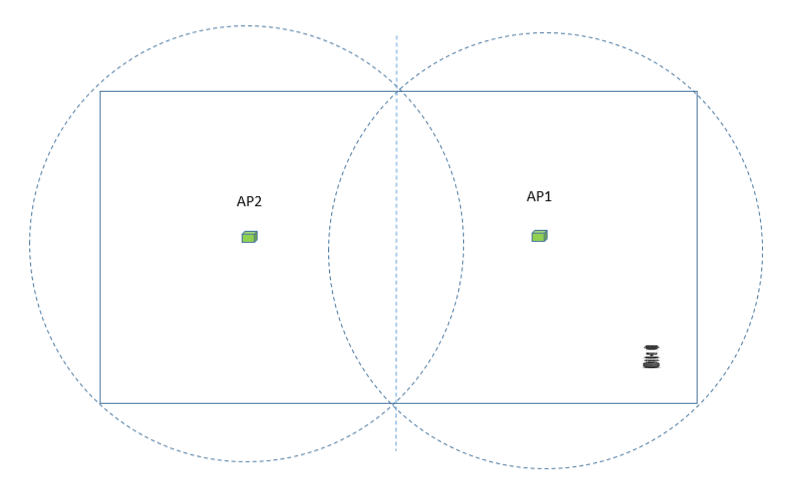
\includegraphics[width=\textwidth, height=0.6\textwidth]{images/w1.png}
		\label{subfig:a} 
		\caption{}
	\end{subfigure}
	\begin{subfigure}[b]{0.495\textwidth}
		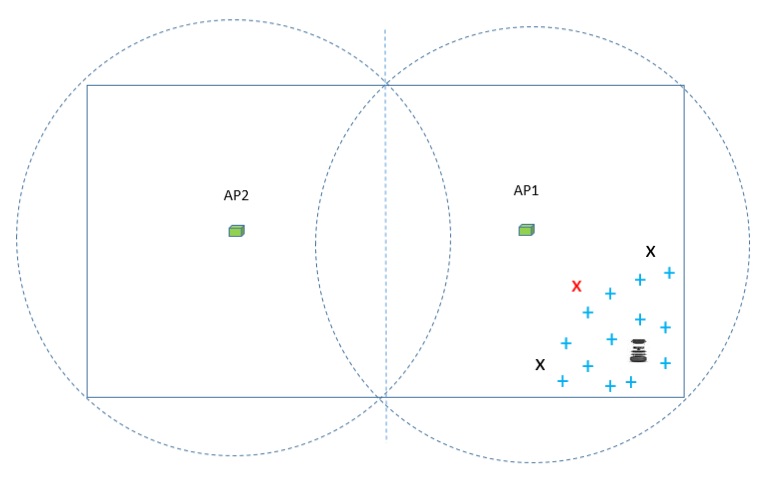
\includegraphics[width=\textwidth, height=0.6\textwidth]{images/w2.png}
		\label{subfig:b}
		\caption{}
	\end{subfigure}
	\begin{subfigure}[b]{0.495\textwidth}
		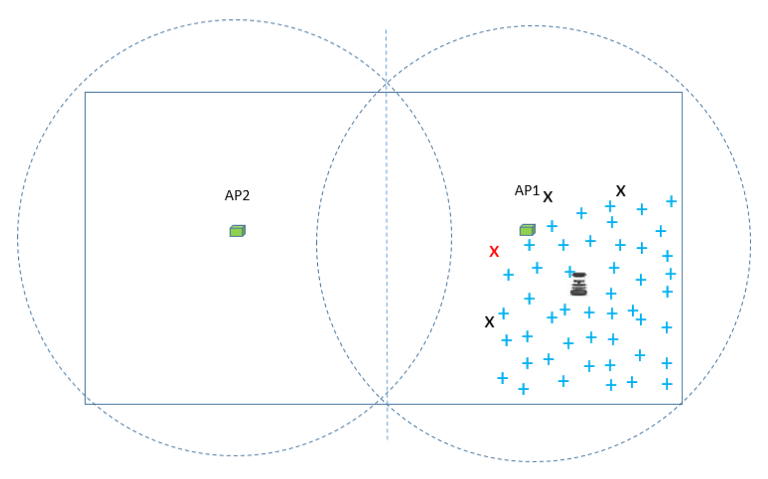
\includegraphics[width=\textwidth, height=0.6\textwidth]{images/w3.png}
		\label{subfig:c} 
		\caption{}
	\end{subfigure}
	\begin{subfigure}[b]{0.495\textwidth}
		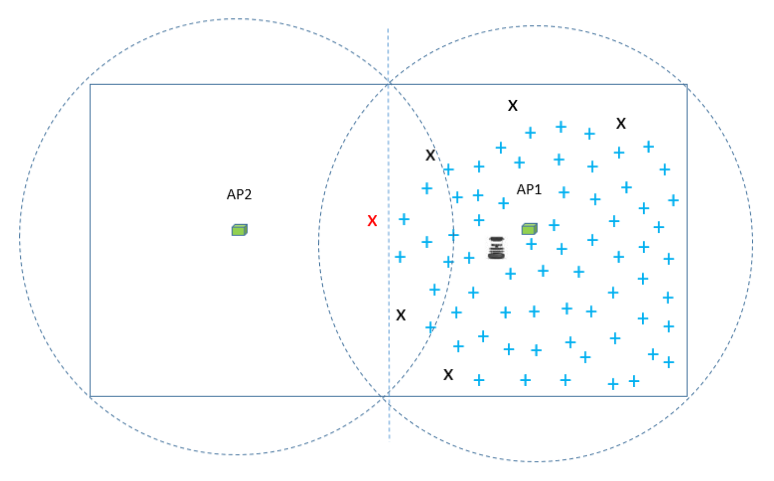
\includegraphics[width=\textwidth, height=0.6\textwidth]{images/w4.png}
		\label{subfig:d}
		\caption{}
	\end{subfigure}
    \begin{subfigure}[b]{0.495\textwidth}
		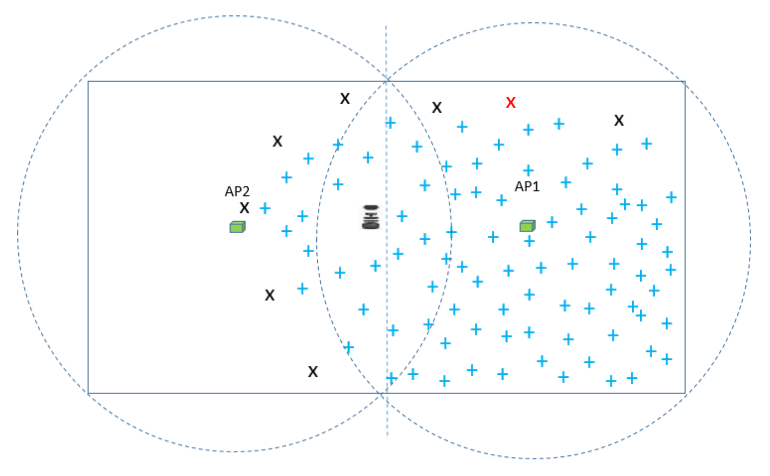
\includegraphics[width=\textwidth, height=0.6\textwidth]{images/w5.png}
		\label{subfig:e} 
		\caption{}
	\end{subfigure}
	\begin{subfigure}[b]{0.495\textwidth}
		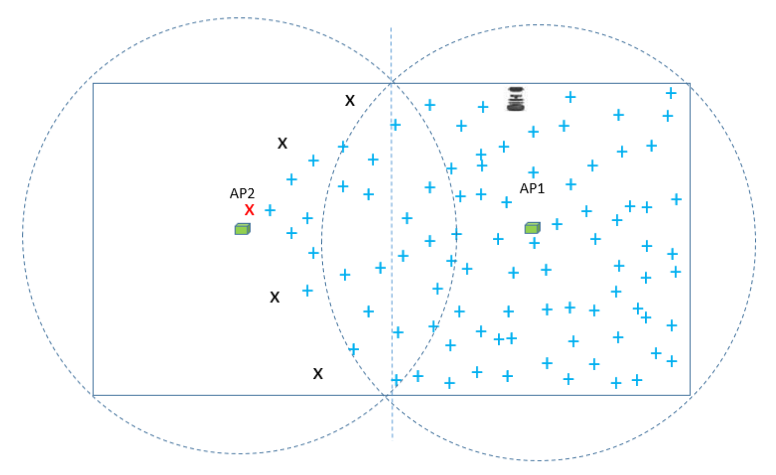
\includegraphics[width=\textwidth, height=0.6\textwidth]{images/w6.png}
		\label{subfig:f}
		\caption{}
	\end{subfigure}
    \begin{subfigure}[b]{0.495\textwidth}
		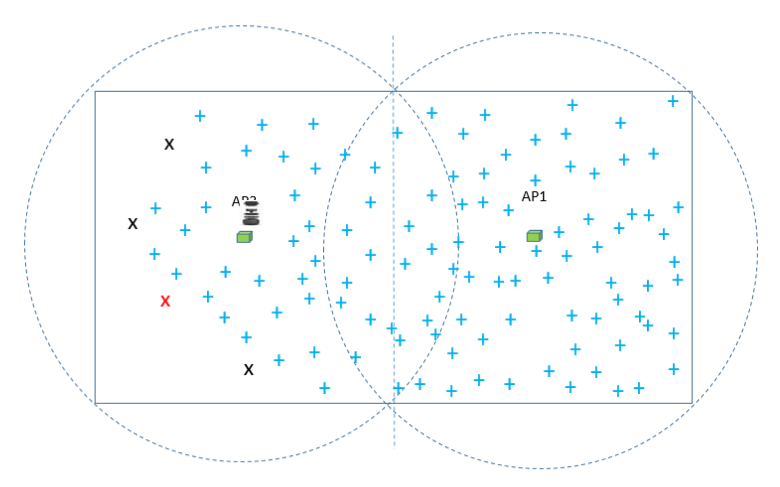
\includegraphics[width=\textwidth, height=0.6\textwidth]{images/w7.png}
		\label{subfig:g} 
		\caption{}
	\end{subfigure}
	\begin{subfigure}[b]{0.495\textwidth}
		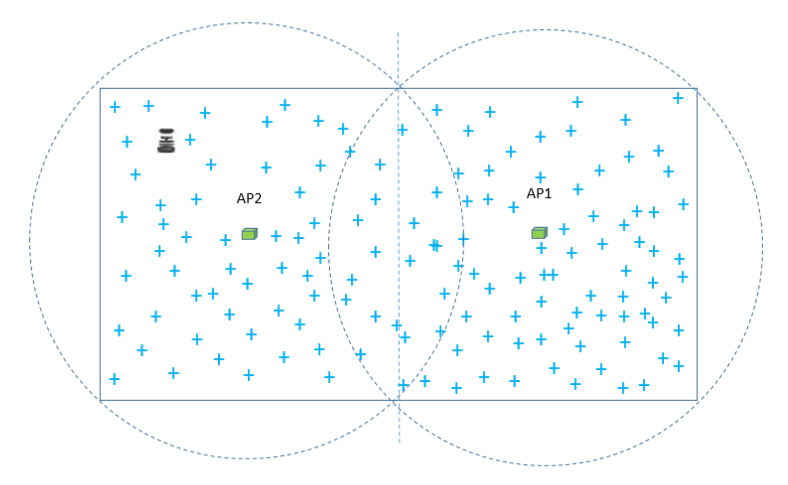
\includegraphics[width=\textwidth, height=0.6\textwidth]{images/w8.png}
		\label{subfig:h}
		\caption{}
	\end{subfigure}
\caption{Illustration of Wi-Coverage in a rectangular space with two access points. + - explored area, x(black) - frontiers identified, x(red) - frontier picked, AP1 and AP2 are access points}
\end{figure*}

\par The robot does an initial Wi-Fi scan and initializes expoAP, which holds the cluster ID(AP ID itself) being explored,to the strongest AP ID which we call the dominant AP. A $360^o$ sensor sweep is performed by the robot and frontiers are obtained using the above explained method exploring partially the environment as shown in Fig 3.2 (A). The explored space is represented in '+' and the white space in the environment represents the area to be explored. The frontier poses are then processed through a Priority Queue which heaps them based on their respective information gain and are associated to currdomAP, the current dominant AP. The Queuer then pops the best frontier associated with expoAP shown in red 'x' and the robot plans its path and moves to it. The robot performs a Wi-Fi scan along with the sensor sweep. If the current dominant AP is same as expoAP, new frontiers are queued and associated with the same AP repeating the above process as illustrated in Fig 3.2 (C) and (D). The robots continues to explore the same fashion until it finds itself sensing better of another AP apart from expoAP as shown in Fig 3.2 (E). Here the Turtlebot crosses the imaginary line of dominance and experiences a stronger signal strength from AP2 and hence the current dominant AP is changed to AP2 ID while expoAP remains unchanged. At this juncture, all new frontiers detected after the sensor sweep are queued in to the Priority Queue and are associated to the currdomAP which is this time, AP2. The frontier popped by the queuer is associated with expoAP i.e AP1 and has the highest of information gains compared to its members. Hence the robot instead of visiting a frontier else where, it visits the frontiers remaining in the partially explored cluster as shown in the Fig 3.2 (F). This continues until all the frontiers associated with expoAP are visited thereby completely exploring the cluster. It is important to note that all new frontiers identified while exhausting the current cluster are associated with their respective cluster numbers along with their information gains. Also the cost to visit the frontiers which are already queued are always updated at each sensor sweep. Once all frontiers corresponding to expoAP are exhausted, it is updated to another cluster ID whose sum of expected gains of all its  frontiers are the maximum. In this case its updated to AP2 ID which is the only remaining cluster. The frontier popped is visited as shown in Fig 3.2 (G) and all new frontiers identified are associated with expoAP, which is now AP2. The process is repeated until all frontiers are visited thereby exploring the entire environment as shown in Fig 3.2 (H). The following is the pseudo-code of Wi-Coverage implementation for a single robot.\\
\vspace{1mm}\\

\noindent\textbf{Algorithm 1: Wi-Coverage using single robot}\\

\begin{algorithm}[H]
% \caption{Wi-Coverage}
\KwData{\\
WiFiC() : get list of AP ids with SS from reachable APs\\
Q() : pushes, pops and heaps}
\textbf{initialize} expoAP \gets $AP\_id\_with\_max\_RSS$\\
\While{no frontiers found}{
\While{!Q(expoAP) is empty}{
O \gets getOccupancyGrid()\;\\
F \gets getFrontiers(G)\;\\
E \gets computeEntropy(F)\;\\
C \gets computeCost(F)\;\\
G \gets computeInfoGain(F)\;\\
Z \gets WiFiC()\;\\
currdomAP \gets getdominantAP(Z)\; \\
Update\_Queue : Q(currdomAP).heap(G, F) \\
nextpose \gets Q.pop(Q(expoAP))\\
}
expoAP \gets $AP\_id\_with\_max(sum(G))$\;\\
}
\end{algorithm}

\vspace{4mm}
\section{Multi-Robot Scenario}
In addition to coverage problem, another reason for the extensive research in autonomous exploration is the benefit that tasks yield when scaling up the number of robots. In many cases multiple robots prove efficient in exploration since huge amounts of time can be saved especially in sizable environments. In case of multiple robots to perform the above discussed frontier exploration, the following should be accomplished for unknown environments.
\begin{itemize}
    \item \textbf{SLAM modules} : Each robot should have its own SLAM module. In other words, they should individually map and localize in their respective local maps.
    \item \textbf{Frontier Detection} : All robots perform frontier exploration for which the frontiers are identified using the above discussed methods. This module is integrated into each robot's controller independently. 
    \item \textbf{Map merging} : As each robot gains information about the environment around itself resulting in a local map, all maps are merged using algorithms such as Graph SLAM\cite{25}.
    \item \textbf{Cluster allocation}: Wi-Coverage works independently on each robot in case of allocating frontiers such that the robot covers the environment cluster by cluster. But in multi robot case, a centralized control is necessary to assign clusters to the robots. This control also checks the number of robots being deployed on the field, especially when the number of robots available are greater than the clusters to be explored.
\end{itemize}

\par When multiple robots are available, clustering the environment online becomes an ultimate advantage. Traditional methods such as cellular decomposition approaches cluster the environment but require complex computations to be performed. Some also expect the robot to remember the visited  spaces which needs storage and solving of necessary edge cases. Wi-Coverage is free from such limitations and prerequisites.      
It can be observed that in case of random frontier allocation, the efficiency of exploration is poor and robots trajectory is completely unpredictive. In a multi robot scenario, though robot coordination becomes easier since the basic criteria of "no two robots get the same frontier" is only to be followed, this strategy still performs poor since robots generally end up with longer trails. Also the number of robots effect the exploration time and computation cost.

\begin{figure*}
    \begin{subfigure}[b]{0.495\textwidth}
		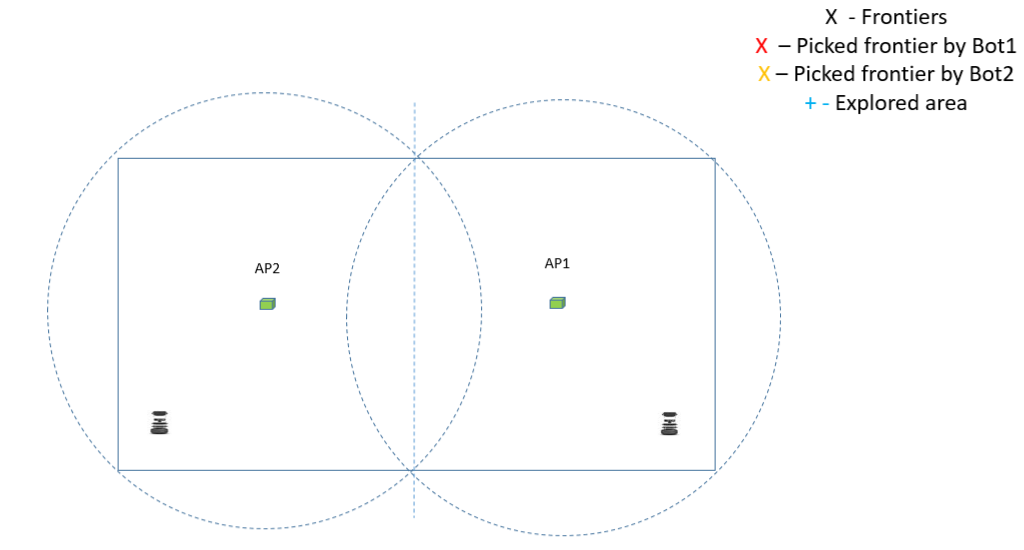
\includegraphics[width=\textwidth, height=0.6\textwidth]{images/wm1.png}
		\label{subfig:a} 
		\caption{}
	\end{subfigure}
	\begin{subfigure}[b]{0.495\textwidth}
		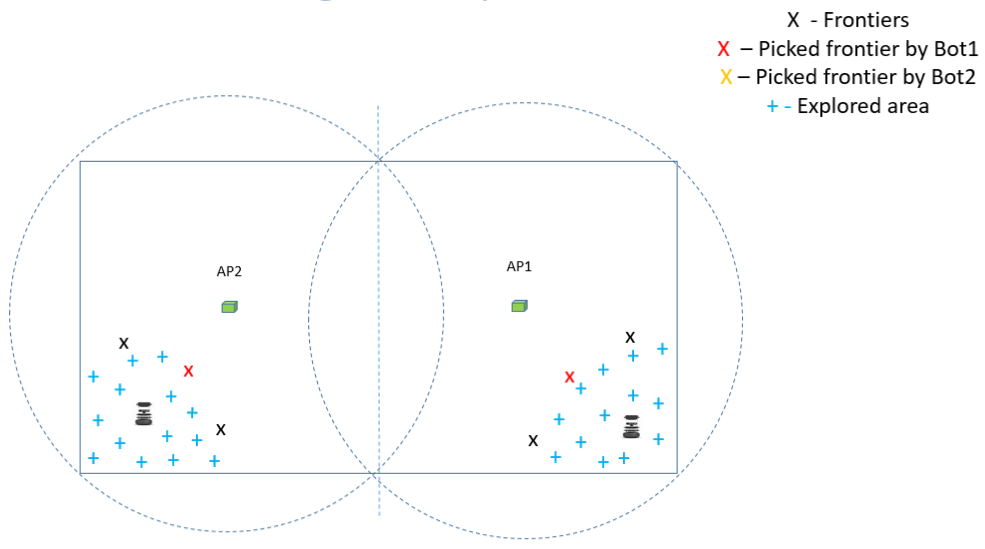
\includegraphics[width=\textwidth, height=0.6\textwidth]{images/wm2.png}
		\label{subfig:b}
		\caption{}
	\end{subfigure}
	\begin{subfigure}[b]{0.495\textwidth}
		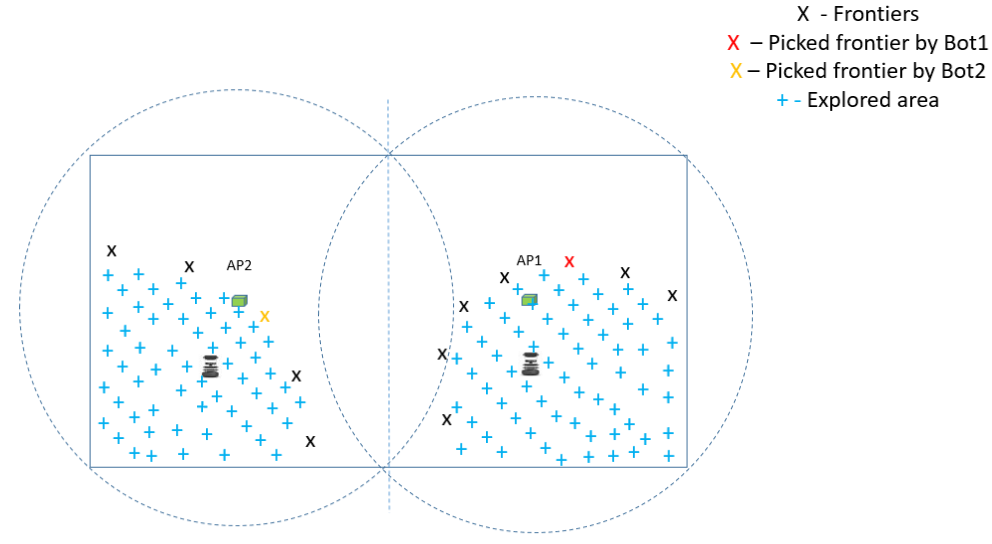
\includegraphics[width=\textwidth, height=0.6\textwidth]{images/wm3.png}
		\label{subfig:c} 
		\caption{}
	\end{subfigure}
	\begin{subfigure}[b]{0.495\textwidth}
		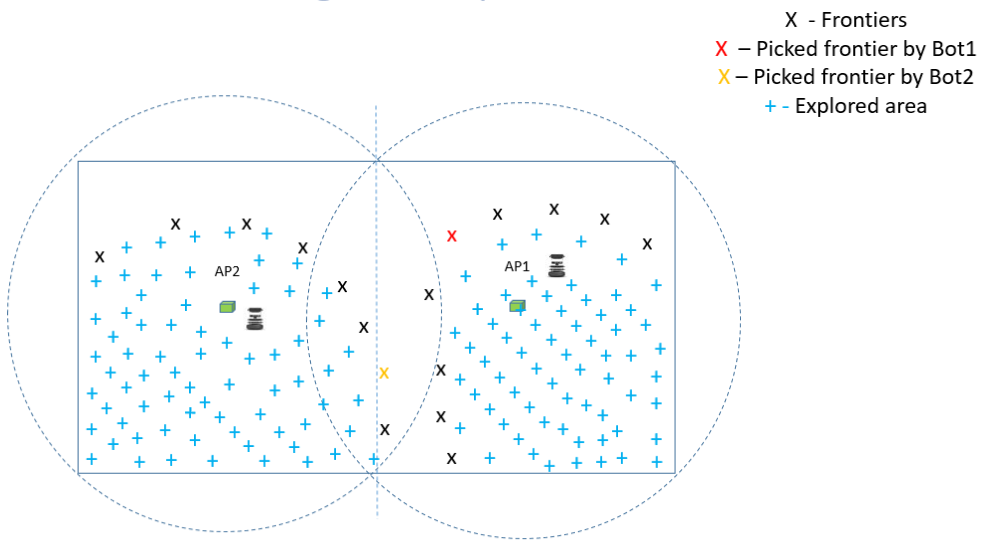
\includegraphics[width=\textwidth, height=0.6\textwidth]{images/wm4.png}
		\label{subfig:d}
		\caption{}
	\end{subfigure}
    \begin{subfigure}[b]{0.495\textwidth}
		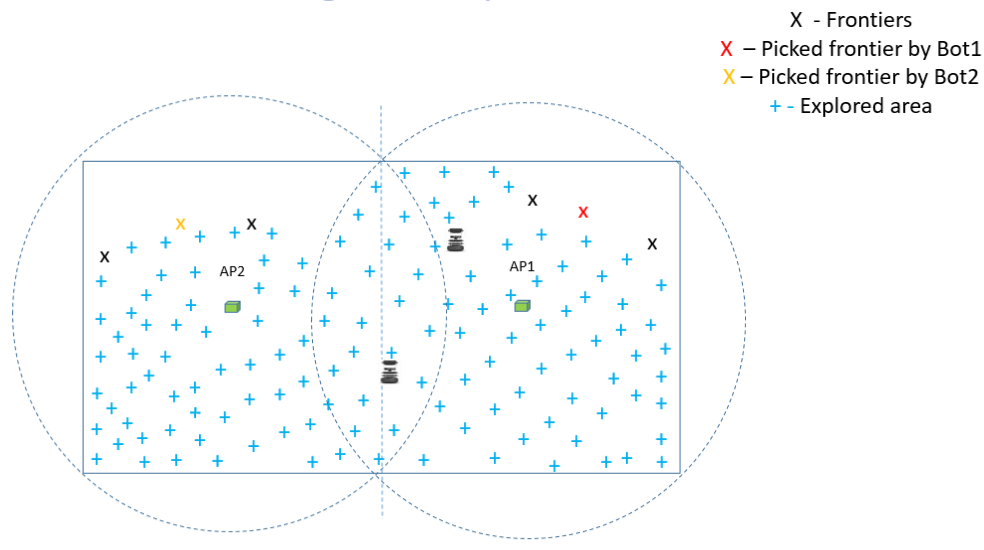
\includegraphics[width=\textwidth, height=0.6\textwidth]{images/wm5.png}
		\label{subfig:e} 
		\caption{}
	\end{subfigure}
	\begin{subfigure}[b]{0.495\textwidth}
		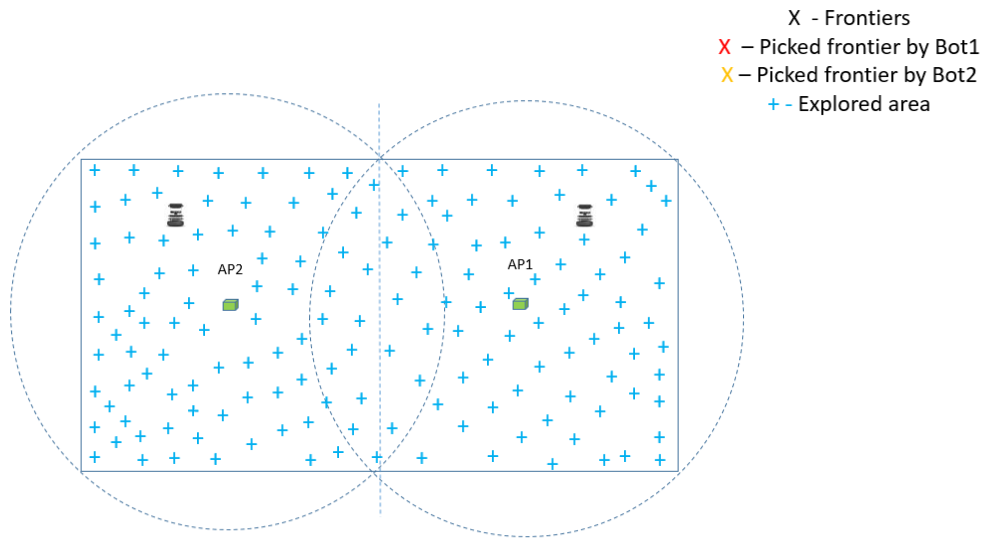
\includegraphics[width=\textwidth, height=0.6\textwidth]{images/wm6.png}
		\label{subfig:f}
		\caption{}
	\end{subfigure}
%     \begin{subfigure}[b]{0.495\textwidth}
% 		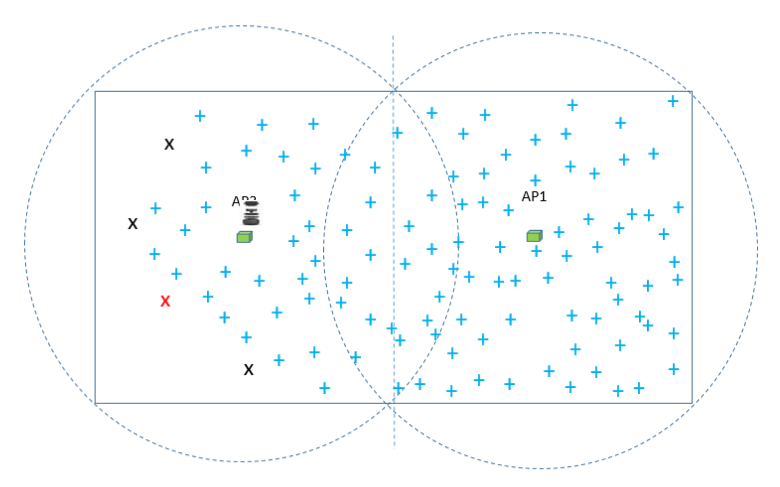
\includegraphics[width=\textwidth, height=0.6\textwidth]{images/w7.png}
% 		\label{subfig:g} 
% 		\caption{}
% 	\end{subfigure}
% 	\begin{subfigure}[b]{0.495\textwidth}
% 		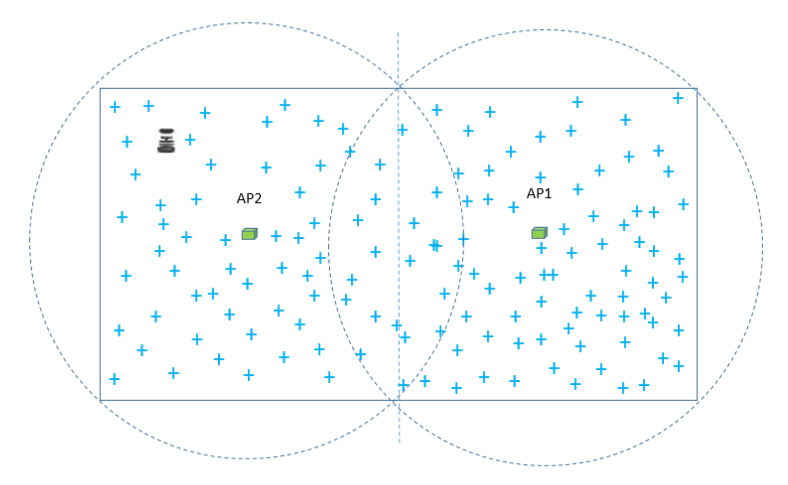
\includegraphics[width=\textwidth, height=0.6\textwidth]{images/w8.png}
% 		\label{subfig:h}
% 		\caption{}
% 	\end{subfigure}
\caption{Illustration of Wi-Coverage with multiple robots in a rectangular space with two access points.}
\end{figure*}

In case of multi-robots, Wi-Coverage has various advantages over other traditional methods.
\begin{itemize}
    \item \textbf{Coordination strategy}: In traditional coverage strategies, the robots need to communicate their poses and the local maps they have explored which can be represented by various metrics(see Chapter 2). In general, these maps, especially the point clouds are data rich and transferring such data takes a toll on the network. Though converting them to relatively simpler structures like graphs or Voronoi diagrams would help reduce the traffic in the network, additional nodes are required to process them continuously. Also as the environment grows larger, the transfers become costly.
    
    \item \textbf{Resource management}: Most coverage methods have a generic strategy which uses all the available robots to explore the environment. Using such methods in scenarios where resources are abundant than required, needs special actions of not exploiting them. Wi-Coverage takes into consideration such requirements by allowing only sufficient work force rather than deploying all the available robots on the field. 
\end{itemize}

To describe Wi-Coverage in a multi-robot scenario, consider the previous environment shown in Fig 3.2(A) but with two robots placed in the environment as shown in Fig 3.3(A). Each robot is equipped with the same sensors, a controller and a motion planner. A master robot allocates clusters to all the robots in the environment. It also decides whether a robot is to be deployed for exploration on the field. Once a robot is allocated a cluster, it explores the environment using Wi-Coverage described in Algorithm 1. 
\par After an initial scan for Wi-Fi APs, the master robot which we call the Allocator gets updated of the total number of APs listened to. It then assigns a cluster to each robot based on its dominant AP. In our example, Robot 1 to the right is assigned cluster AP1 and Robot 2 is assigned cluster AP2 since they are the corresponding dominant APs they listen to. The Allocator maintains a record of the allocated clusters and unallocated clusters in the environment. The robots then perform exploration using Wi-Coverage in their respective clusters as shown in the Fig 3.3 (C),(D) and (E). Once the clusters are explored, the Allocator is updated by sending a feedback message from each robot. If any unexplored cluster is available, the Allocator assigns the cluster to the robot which listens to the corresponding AP, the strongest. Algorithm 2 below shows a pseudo-code for Wi-Coverage using multiple robots.
% \clearpage
\vspace{1.5em}

\noindent\textbf{Algorithm 2: Wi-Coverage using multiple robots}

\begin{algorithm}[H]
% \caption{Wi-Coverage}
\KwData{\\
WiFiC() : gets AP ids with SS of reachable APs\\
Q() : pushes, pops and heaps\\
Allocator() : Assigns clusters}
\textbf{initialize};
clusterlist \gets UnionOfAPidsSensed\\
\While{!clusterlist is empty}{
\For{each bot}{
    bot(expoAP) \gets Allocator() assigns cluster_i\\
    \While{$!cluster_i$ is explored}{
        do \textbf{Algorithm 1}\\
    }
    clusterlist \gets delete $cluster_i$\\
    \If {new AP detected}{
    clusterlist \gets $new\_cluster$\\
    }
}
}
\end{algorithm}

\vspace{1.5em}

\par The Allocator also considers situations when more than one robot gets the same cluster to be explored. This happens when robots share the same dominant AP, i.e when they start from the same cluster. In such case, the robot which listens stronger to the AP gets the current cluster and the other bot(s) get(s) the cluster(s) to which it(they) listen the best apart from the current AP as shown in Algorithm 3 below.

\vspace{1.5em}

\noindent\textbf{Algorithm 3: Cluster allocation}

\begin{algorithm}[H]
% \caption{Wi-Coverage}
% \KwData{\\
% % Allocator() : tracks cluster allocation
% N : Number of robots}
\While{no frontiers found}{
\For{each update}{
    % \For{i=1\,1$<$N-1}
    \If{bot_i(expoAP)~ $==$~ bot_{j}(expoAP)}{
        min(SS_i,SS_{j}) \gets $corresponding\_next\_best\_domAP$\;\\
    }
}
}
\end{algorithm}

Algorithm 4 shows a psuedo-code describing the frontier selection of a robot in seek of the cluster assigned. In the above scenario where robots start from same dominant AP region, the robot which is assigned another cluster selects frontiers such that it moves towards by tracking the signal strength.\\

\noindent\textbf{Algorithm 4: Cluster search when bots start from same location}

\begin{algorithm}[H]
% \caption{Wi-Coverage}
\KwData{\\
\%SS(): gets percentage signal strength}
\While{!\%SS(expoAP) $>$ 0}{
nextpose \gets maximize(SS(Q.pop(Q(domAP))))\;\\
}
\end{algorithm}

If no unexplored clusters are available and all which were assigned are explored, the exploration is said to be complete as shown in Fig 3.3(F). The maps from each robot are then merged using Graph SLAM.
To summarize, the robots perform exploration using Wi-Coverage individually in clusters assigned by the Allocator. Since the robots need not know each others positions, the only information transferred between the robots is merely a cluster id while allocating clusters. This is far less complicated and less communication intensive than other available methods for multi-robot exploration.

% \clearpage

\section{Systems}
This section is about the software and hardware systems used in this work. Hardware design, communication protocols, middleware design and structure and about simulation software, Gazebo are discussed.  

\lhead{\emph{Systems}}
\subsection{Hardware and low-level drivers}
The lowest layer of system abstraction is the hardware. The motorized wheel, all hard connections which carry power and data in and around the robot, the sensor payloads and the batteries come under this.
Sensors communicate using various protocols and over different hardware interfaces. The interface between low-level drivers and the middleware translates the raw data from the sensors into a common format which is used by other consequent processes.

\begin{figure}[!b]
    \centering
    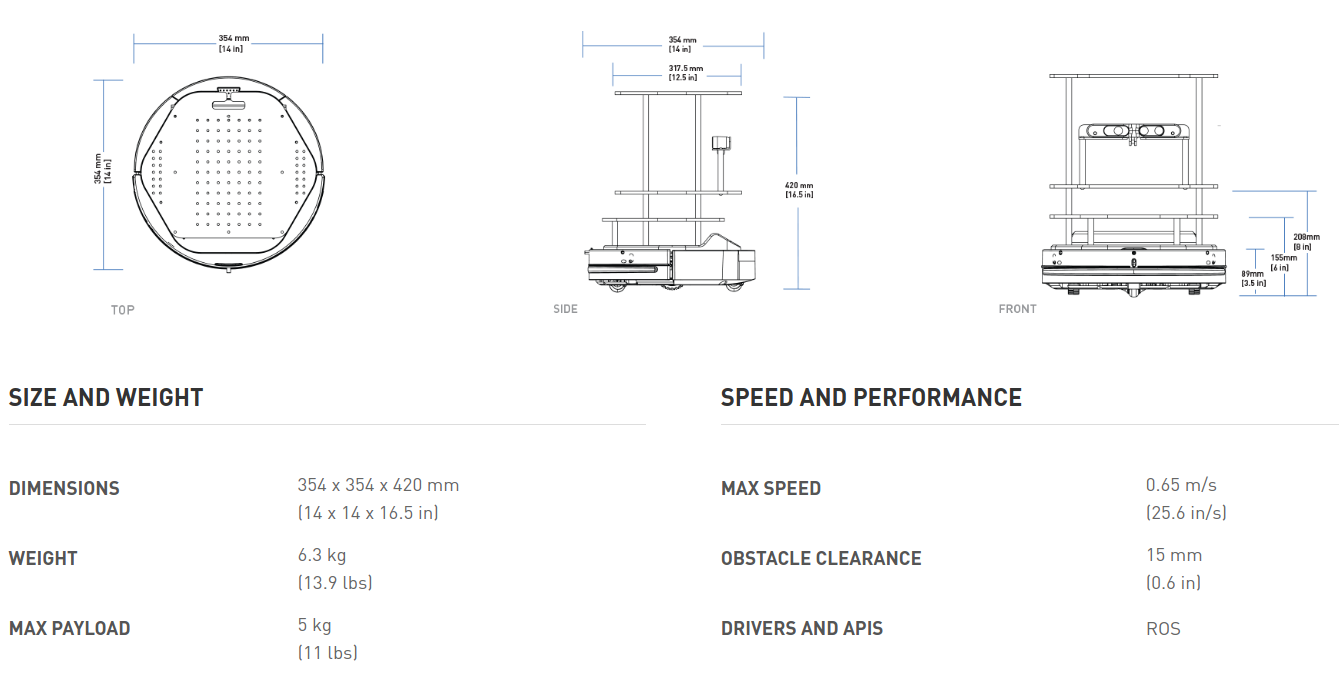
\includegraphics[width=\textwidth]{images/botspecs.png}
    \caption{Turtlebot 2 technical specifications. Image courtesy \cite{41}}
    \label{fig:tb}
\end{figure}

\subsubsection{Darwin}
Our robot, Darwin, which we choose to make it into an autonomous explorer is a Turtlebot 2. Turtlebots are low-cost, personal robot kits with open-source software created by Willow Garage by Melonee Wise and Tully Foote\cite{32}. Darwin is the next and improved version of the first generation Turtlebot developed by Clearpath Robotics. A Turtlebot has been built for ROS and supports all major packages out of the box. As with many other ROS platforms, one of the biggest strengths of the Turtlebot is the support community. Fig 3.4 below lists the specifications of the robot. Darwin is equipped with an Yujin Kobuki mobile base, a Kinect Xbox 360 sensor, an Nvidia TK1 CPU which contains our code base, fast charger and a 2200mAh battery pack. It also comes with a fast charging dock that Turtlebot can autonomously dock with. All low level drivers that handle wheel motors, encoders and other communication protocols are built-in.

\section{Middleware and High-level applications}
The low-level hardware such as motors or cameras and high-level applications such as motion planning or object recognition are integrated by a middleware. It is a software layer facilitating communication between them which is required for modularising components in a robot system.   

\subsection{ROS: Robot Operating System}
Nowadays autonomous Robots are getting more and more complex, using various types of sensors and motors\cite{20}. Therefore the demand for a framework that integrates the sensors and all the hardware components of the robot with an operating system is quite high. Another need for the community is code re-usability. ROS is an open source framework\cite{13} that aids in development of various robot applications. It serves as a platform which eliminates the work of building an application from scratch by providing various low level drivers and communication protocols. It makes a developer's work much easier and focused on the core application and saves considerable amount of time. Apart from offering quality applications as packages which are a run and play type, it hosts a great community which helps solve problems.
\par ROS is also popular as a meta-operating system that provides tools and libraries to help the users develop complex robotic applications. It supports parallel computing and distributed communication framework. The individual components in an application can interact using ROS without being constrained to run on a single computer. Although there are various robot frameworks such as Player, YARP, Orocos, CARMEN, Orca, MOOS, and Microsoft Robotics Studio available, ROS has gained attention due to its distributed nature, code re-usability and community support.

\subsection{ROS Levels}
ROS uses divide and conquer method while designing complex robot applications\cite{34}. Nodes are the fundamental components of ROS. These are individual executables which communicate with each other through messages using topics as shown in Fig 3.6. Though ROS is not a full fledged operating system, the primary idea behind this is to emulate such behavior while promoting code reuse and distributed networking. Nodes are contained in a package and packages with common goal are grouped as stacks such as navigation stack. Each package has a manifest(\textit{package.xml}) that describes its functionality and dependencies on other packages. Fig 3.5 represents the communication framework of ROS\cite{33}.
The following describe various levels and components in ROS framework.

\begin{figure}[!b]
    \centering
    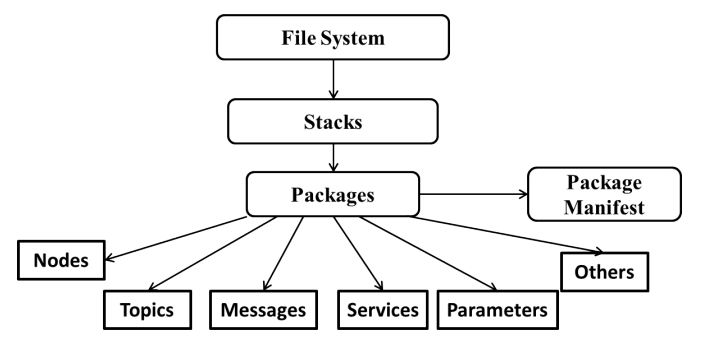
\includegraphics[width=\textwidth]{images/ros1.png}
    \caption{ROS as an ecosystem. Image from \cite{49}}
    \label{fig:r1}
\end{figure}

\begin{figure}[!b]
    \centering
    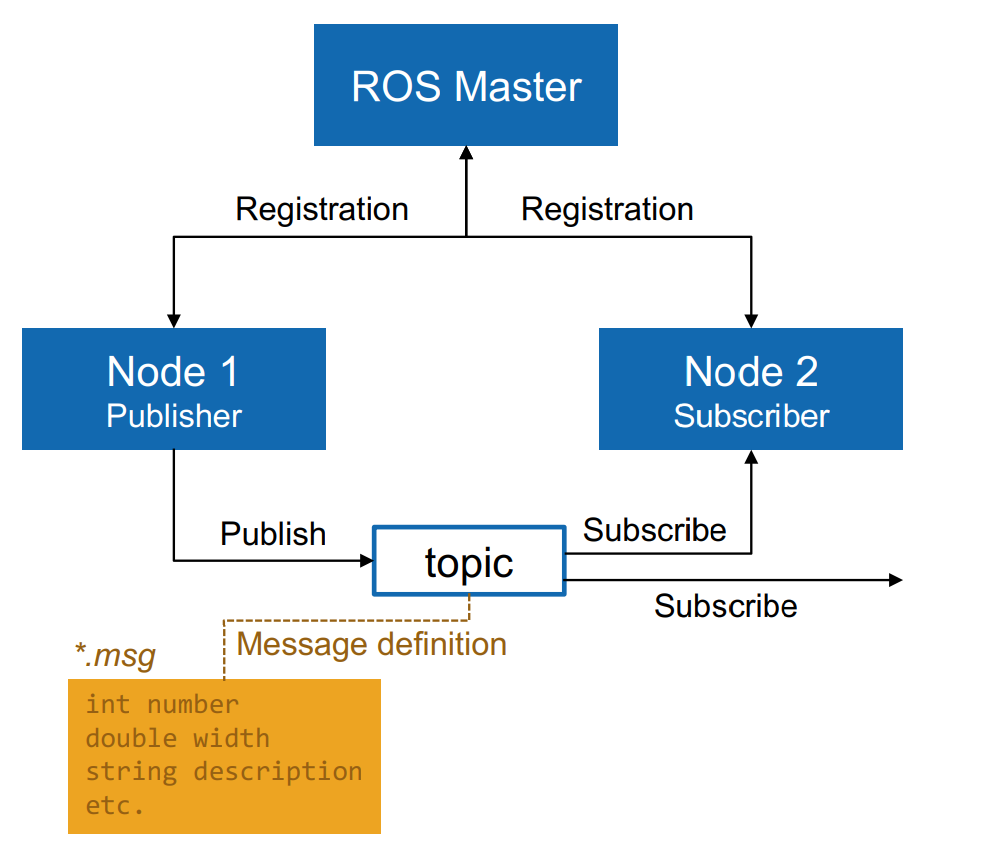
\includegraphics[width=0.75\textwidth]{images/ros2.png}
    \caption{Basic communication framework in ROS. Image from \cite{48}}
    \label{fig:r2}
\end{figure}

\subsubsection{File System Level}
\begin{itemize}
    \item Packages: These constitute the main unit for organizing software in ROS\cite{48}.
    \item Manifests: These provide metadata about a package, including its license information and dependencies, as well as language specific information such as compiler flags.
    \item Stacks: Collection of packages that provide aggregate functionality.
    \item Stack manifests: Similar to package manifests but provides data of the stack.
    \item Message: These are descriptions that define data structures for messages sent in ROS.\\ Example: \textit{my\_package/msg/MyMessageType.msg}.
    \item Service: These descriptions define the request and response data structures for services in ROS. This establishes a request and acknowledgement protocol between nodes to communicate efficiently. Example: \textit{my\_package/srv/MyMessageType.srv}.
\end{itemize}

\subsubsection{Computation Graph Level}
\begin{itemize}
    \item Nodes: Nodes are combined graphs which communicate via streaming topics, services and parameter server\cite{33}.
    \item ROS Master: This provides naming and registration services to the rest of the nodes in ROS system.
    \item Parameter Server: It is a shared, multi-variate dictionary that is accessible via network APIs. The parameter server is implemented using XMLRPC and runs inside of the ROS Master, which means that its API is accessible via normal AMLRPC libraries\cite{33}.
    \item Topics: These are named buses over which nodes exchange or share messages based on publish/subscribe policy.
    \item Bags: A format for saving and playing back ROS message data.
\end{itemize}

\subsection{Gazebo: Simulator}
Robot simulation is an essential tool in every roboticist's toolbox. A well-designed simulator makes it possible to rapidly test algorithms, design robots, perform regression testing, and train AI system using realistic scenarios. Gazebo\cite{18} is a 3D dynamic simulator with the ability to accurately and efficiently simulate populations of robots in complex indoor and outdoor environments. While similar to game engines, Gazebo offers physics simulation at a much higher degree of fidelity, a suite of sensors, and interfaces for both users and programs. The key features of Gazebo include\cite{18} multiple physics engines, a rich library of robot models and environments, a wide variety of sensors and convenient programmatic and graphical interfaces. Fig 3.5 above shows the building editor of Gazebo which just requires a blueprint of the environment to be created. Fig 3.8 shows the environment designed using the building editor. A blue print of the building was used and all measurements are to scale. Different colors are given to walls for better visual distinction. 

\begin{figure}
    \centering
    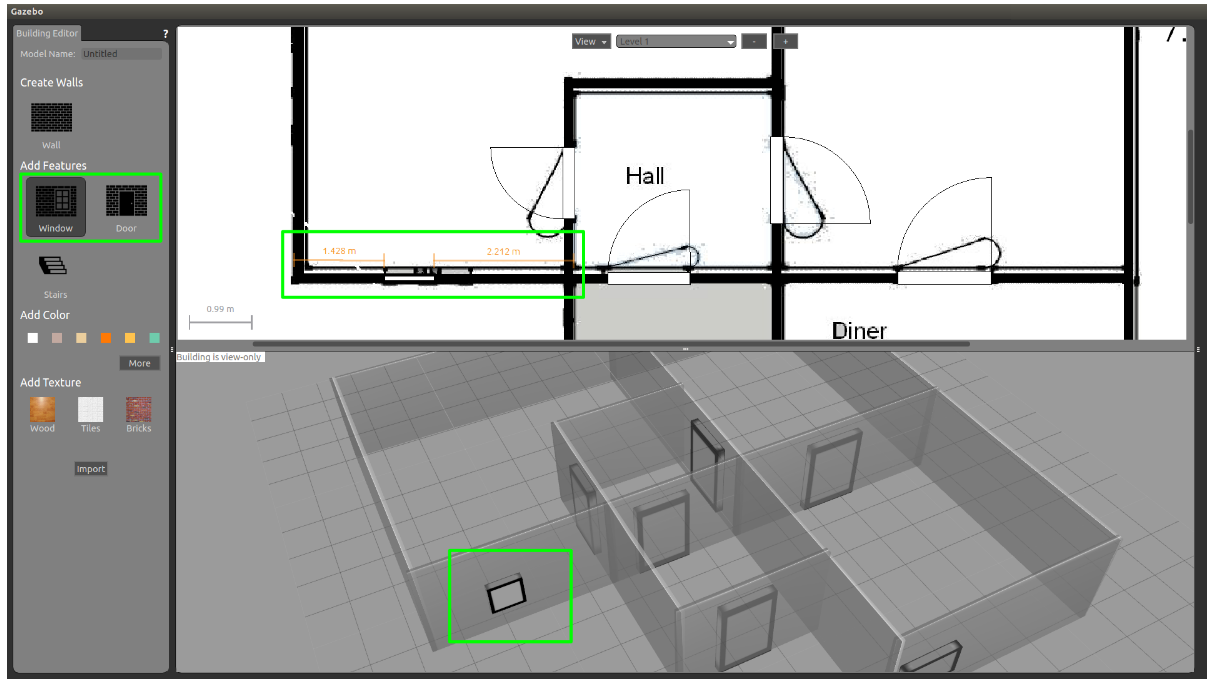
\includegraphics[width=\textwidth]{images/gazebo2.png}
    \caption{A snapshot of Gazebo simulator GUI. The interface shows the building editor where the top section is the blueprint and below is the environment being built using it.}
    \label{fig:gazebo}
\end{figure}

\begin{figure*}[!h]
    \begin{subfigure}[b]{\textwidth}
		\centering
		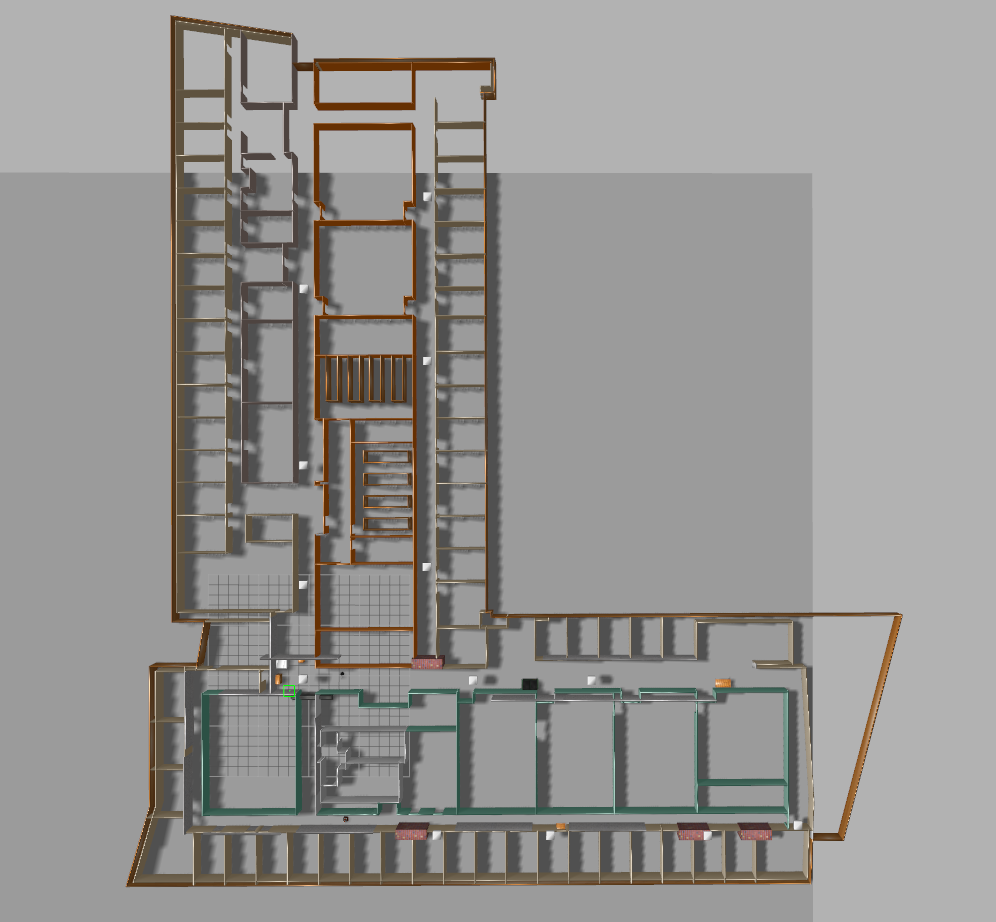
\includegraphics[width=0.49\textwidth]{images/davis3g1.png}
		\label{subfig:a}
		\caption{}
		\vspace{2em}
	\end{subfigure}
	\begin{subfigure}[b]{\textwidth}
	    \centering
		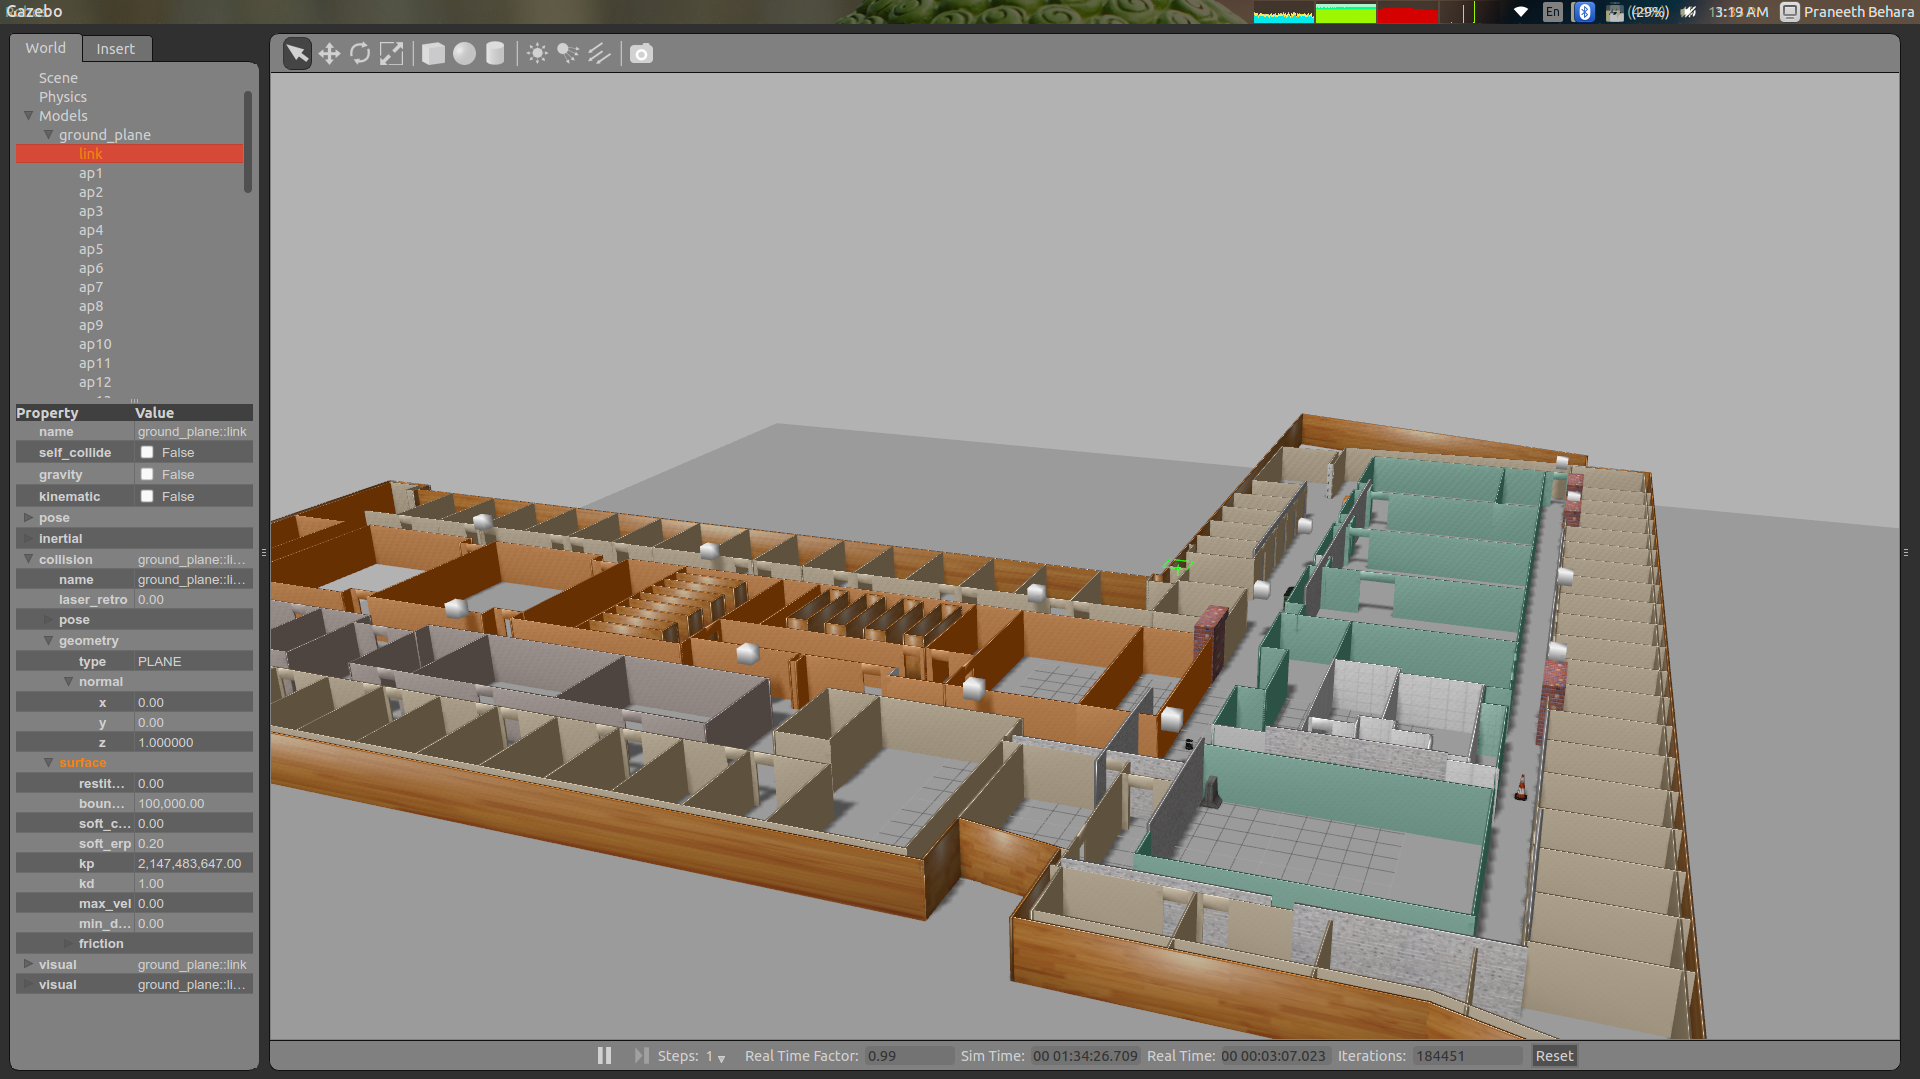
\includegraphics[width=0.49\textwidth]{images/davis3g2.png}
		\label{subfig:b}
		\caption{}
	\end{subfigure}
\caption{Shows a 100x80m to scale simulation environment of Davis Hall, UB, created using Gazebo building editor for this work.}
\end{figure*}

% \subsubsection{SDF}

% \subsection{RTAB-Map}

\subsection{Tools and Packages used}
ROS modules and packages which were used for SLAM and navigation are described below. Also other tools which help maintain the huge code base and help visualize and debug are mentioned as well. 

\textbf{RTAB-Map}: Real-Time Appearance-Based Mapping\cite{50} is a RGB-D SLAM approach based on a global loop closure detector with real-time constraints. This package can be used to generate a 3D point clouds of the environment and$/$or to create a 2D occupancy grid map for navigation. It has a Graph SLAM approach based on a global Bayesian loop closure detector. A bag-of-words approach is used to determine how likely a new image comes from an already visited location or a new one. A new constraint to the map's graph is added when a loop closure hypothesis is accepted. A graph optimizer then minimizes the errors in the map. To limit the number of locations used for loop closure detection and graph optimization, a memory management approach with short-term and long term memories are used. RTAB-Map can be used alone with a hand-held Kinect or stereo camera for 6DoF RGB-D mapping, or a laser rangefinder for 3DoF mapping. \url{http://wiki.ros.org/rtabmap} 

\textbf{move\_base}: This package helps in moving the robot to desired positions in the map using ROS navigation stack. It uses the actionlib package to achieve the above through actions. The move\_base node links together a global and local planner to accomplish its global navigation task. \url{http://wiki.ros.org/move_base}

\textbf{RViz}: 3D visualization tool for ROS. Used to display 3D sensor data, exploration trajectories, maps and to handle user input. \url{http://wiki.ros.org/rviz} 

\textbf{Gitlab}: A version control software which stores code base, tracks any changes made and helps maintaining multiple version for switching and testing. It also allows group sharing and collaboration. \url{https://gitlab.com}